\documentclass{beamer}   % class
\usetheme{Warsaw}    % style
\usecolortheme{default}   % color
\setbeamercovered{transparent}
\title[priyankacool10.wordpress.com]{e-Notice App}
\subtitle{An Android Application}
\author[Guru Nanak Dev Engineering College]{Priyanka Kapoor \\ 100371180720}
\begin{document}
\frame{\titlepage}

\begin{frame}
\begin{block}{Mentor}
Er. Rustam Singh\\
Associate Software Developer at DigiMantra Labs, Ludhiana
\end{block}
\end{frame}

\begin{frame}
\begin{block}{Problem Description}
To develop a mobile application that will help you receiving the notices from the college, anywhere, anytime. Earlier their was problem that notices were pasted on notice board. If there is holiday on the
next day, nobody will be able to read it. Moreover, when there is any notice regarding exams, there is much crowd
in front of notice board. So in order to ease the students as well as staff members, there was a dire need to have
any notice application that can run on mobile phones.
\end{block}
\end{frame}

\begin{frame}
\frametitle{Project Objectives}
\begin{enumerate}
\item Faster dissemination of notices regarding education, technical events, cultural events.\pause
\item Any lost/found going out in college.\pause
\item Easy way to broadcast your message.\pause
\item Helps you to be updated with whats going on in College.\pause
\item Good way to advertise about Tuitions/Coaching Courses.\pause
\end{enumerate}

\end{frame}

\section{e-Notice App}
\subsection{Introduction}
\begin{frame}
\frametitle{Introduction}
e-Notice App is an Internet based Mobile Application that helps you access college notices on your Android phone. It buzzes you
whenever any notice arrives.
\end{frame}

\section{Design of Project}
\begin{frame}
\frametitle{Design of Project}
\begin{block}{Use Case Diagram}
A Use Case diagram at its simplest is a representation of a user’s interaction with the system and
depicting the specifications of a use case. A use case diagram can portray the different types of users of a
system and the various ways that they interact with the system.
\end{block}
\end{frame}

\subsection{Use Case Diagram for User}
\begin{frame}
\frametitle{Use Case Diagram for User}
\begin{figure}
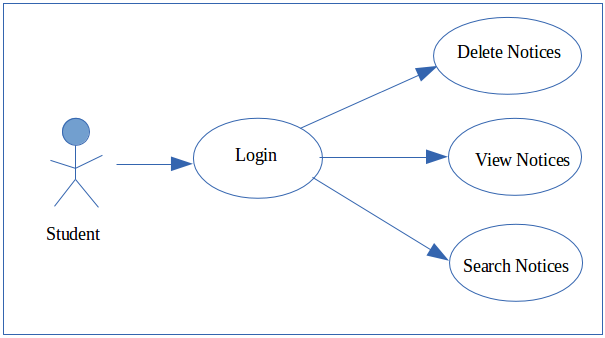
\includegraphics[scale=0.4]{image/usecase1.png}
\caption{Use Case Diagram For User}
\end{figure}
\end{frame}

\subsection{Use Case Diagram for Admin}
\begin{frame}
\frametitle{Use Case Diagram for Admin}
\begin{figure}
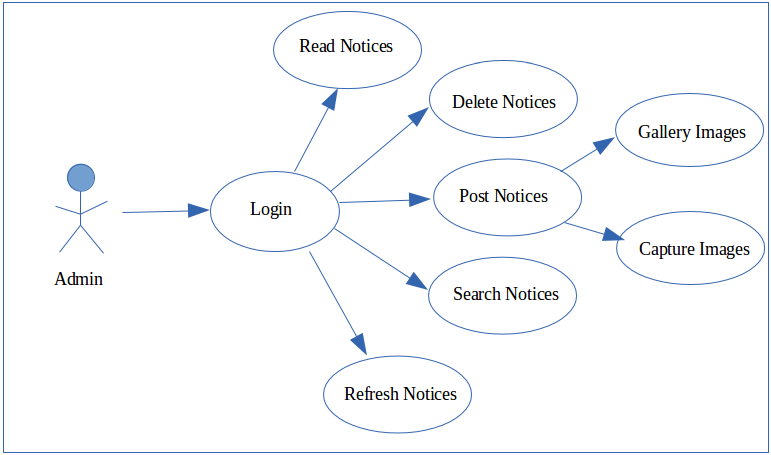
\includegraphics[scale=0.3]{image/usecase2.png}
\caption{Use Case Diagram For Admin}
\end{figure}
\end{frame}

\subsection{Detailed Design}
\begin{frame}
\frametitle{Detailed Design of Project}
\begin{block}{Detailed Design}
Detailed Design of any project depicts the entire working of the project. It answers the following questions:
\begin{itemize}
\item What are the types of user?
\item What are functions performed by project?
\item What is going on behind the scenes?
\item What comes up in front of user? 
\end{itemize}
\end{block}
\end{frame}

\subsection{e-Notice App Design}
\begin{frame}[plain]

\begin{figure}
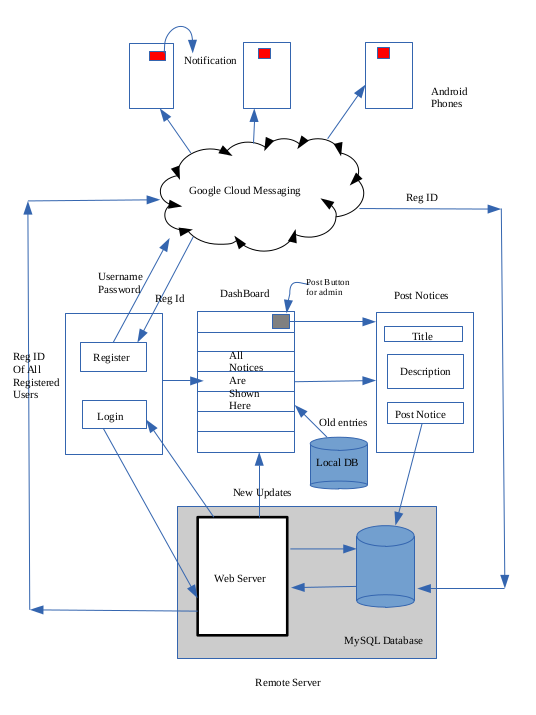
\includegraphics[scale=0.4]{image/detaildesign.png}
\caption{Detailed Design}
\end{figure}
\end{frame}

\section{Project Modules}
\begin{frame}
\frametitle{Project Modules}
\begin{itemize}
\item \textbf{User Interface}\pause
\item \textbf{Communication With Web Server}\pause
\item \textbf{Parsing JSON Responses}\pause
\item \textbf{Services and Broadcasts}\pause
\item \textbf{GCM Notifications}\pause
\end{itemize}
\end{frame}

\subsection{User Interface}
\begin{frame}
\frametitle{User Interface}
User Interface is what comes in front of the user. Its a page or an activity with which a user deals.
Upcoming pages shows up the user interface of the application.
\end{frame}


\begin{frame}
\frametitle{Landing Page}
\begin{figure}
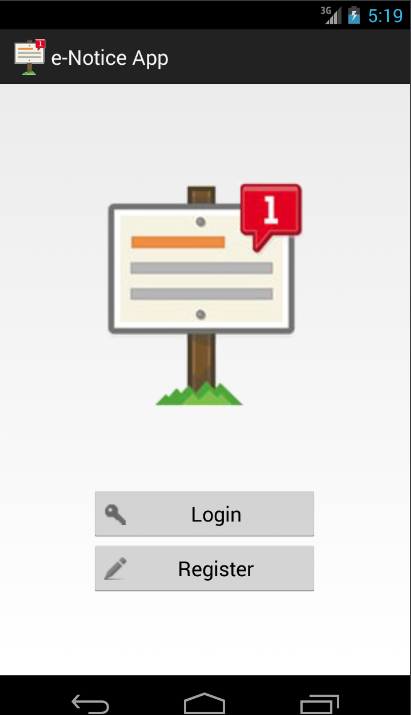
\includegraphics[scale=0.2]{image/landing.png}

\end{figure}
\end{frame}


\begin{frame}
\frametitle{Registration Page}
\begin{figure}
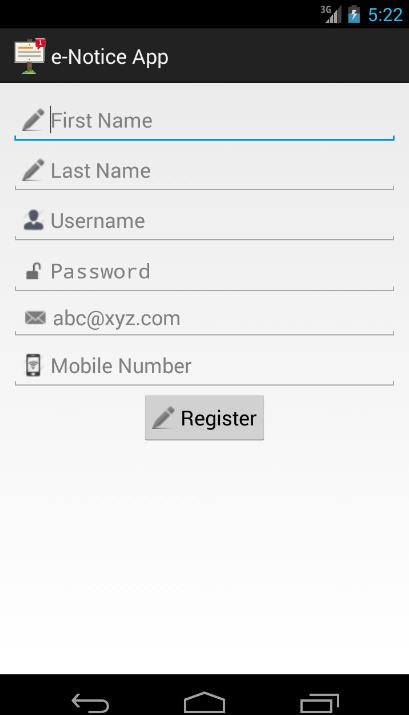
\includegraphics[scale=0.2]{image/register.png}
\caption{Register}
\end{figure}
\end{frame}


\begin{frame}
\frametitle{Login Page}
\begin{figure}
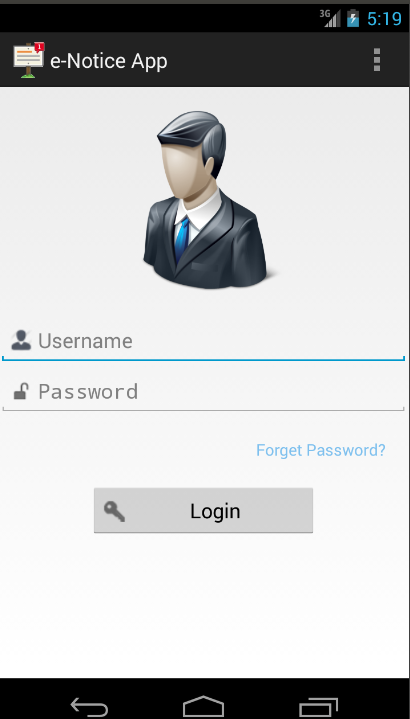
\includegraphics[scale=0.2]{image/login.png}
\caption{Login}
\end{figure}
\end{frame}


\begin{frame}
\frametitle{DashBoard of Notices}
\begin{figure}
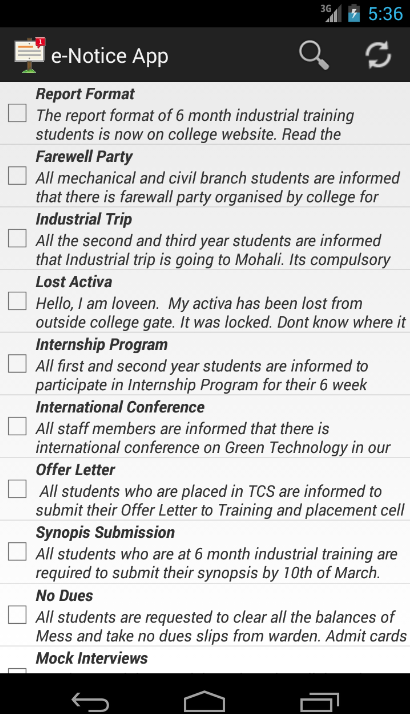
\includegraphics[scale=0.2]{image/dashboard.png}
\caption{Dashboard}
\end{figure}
\end{frame}


\begin{frame}
\frametitle{Admin Panel}
\begin{figure}
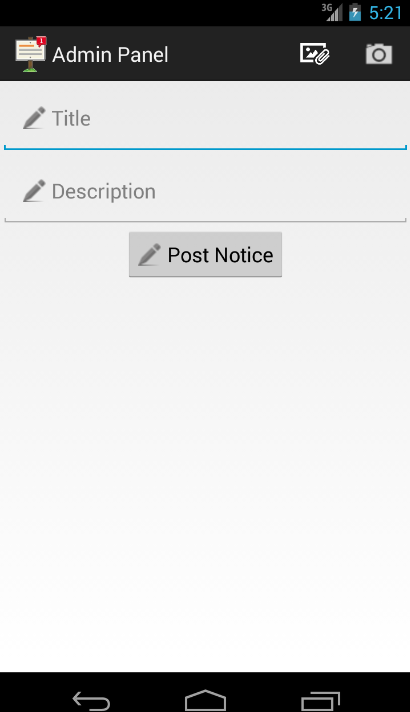
\includegraphics[scale=0.2]{image/post.png}
\caption{Page for Posting Notices}
\end{figure}
\end{frame}

\subsection{Communication With Web Server}
\begin{frame}
\frametitle{Communication With Web Server}
This application is communicating with the Web Server in order to fetch all the notices of the college. It fetches notices from the server
and store it inside its local database. Next time, when the user opens up the application, it fetches the previous data from its local database and fetches only new updates or messages. In this way, it reduces the traffic on the server.

\end{frame}

\subsection{JSON Parsing}
\begin{frame}
\frametitle{JSON Parsing}
JSON stands for JavaScript Object Notation. It is independent data exchange format and is best alternative for XML.
All the Web Server responses are JSON encoded. So the application needs to parse the JSON in order to get the actual response or message from the server. 

\end{frame}

\subsection{Services and Broadcast Receivers}
\begin{frame}
\frametitle{Services}
Service is a process that runs in background to perform long term operations or work for remote processes. Services don't provide a user interface.\\
This application also uses a service whose task is to fetch the message sent by the GCM server and generate notifications of the received messages. This service is called only when broadcast receiver sends a message to it. It is not running continuously all the time. Thus it saves your mobile battery too.
 
\end{frame}

\begin{frame}
\frametitle{Services Screenshot}
\begin{figure}
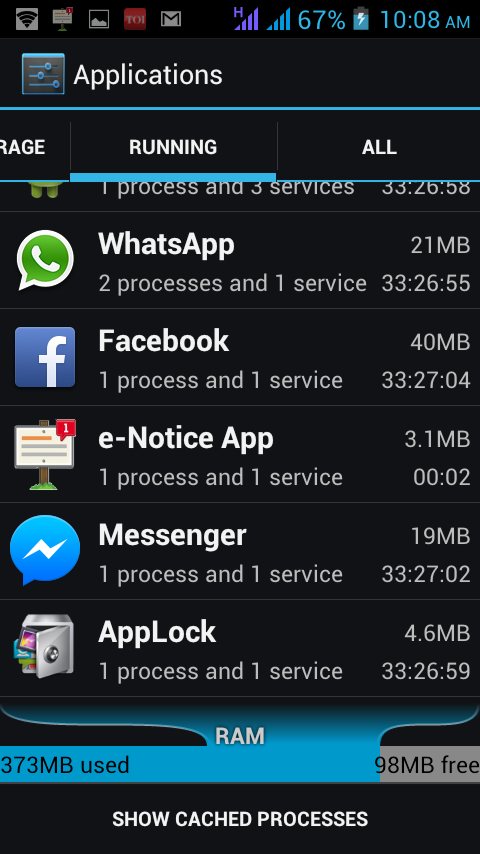
\includegraphics[scale=0.2]{image/service.png}
\caption{Service Running In Application}
\end{figure}

\end{frame}

\begin{frame}
\frametitle{Broadcast Receivers}
Broadcast Receiver is a component that responds to system conditions such as low battery or the screen being turned off.
This application has a broadcast receiver that receives the GCM message and simultaneously run the service in order to generate the 
notification.
 
\end{frame}

\subsection{GCM Notifications}
\begin{frame}
\frametitle{GCM Notifications}
Google Could Messaging (GCM) is a service that allows you to send data from your server to your user's Android-powered device, and also to receive messages from devices on the same connection. GCM is completely free no matter how big your messaging needs are and there are no quotas.
 
\end{frame}

\begin{frame}
\frametitle{How GCM Works?}
\begin{enumerate}
\item Android device sends SENDER\_ID to GCM Server for registration. \pause
\item After successful registration, GCM sends Registration Id to Android device.\pause
\item After getting Registration Id, Android device sends Registration Id to Web Server.\pause
\item Store Registration Id in our database at the server.\pause
\item Whenever Push Notification needed, get Registration Ids from server, and send the request too GCM with Registration Id and message.\pause
\item After push notification request, GCM sends Push Notifications to Android device.
\end{enumerate}
\end{frame}

\begin{frame}
\frametitle{GCM Working}
\begin{figure}
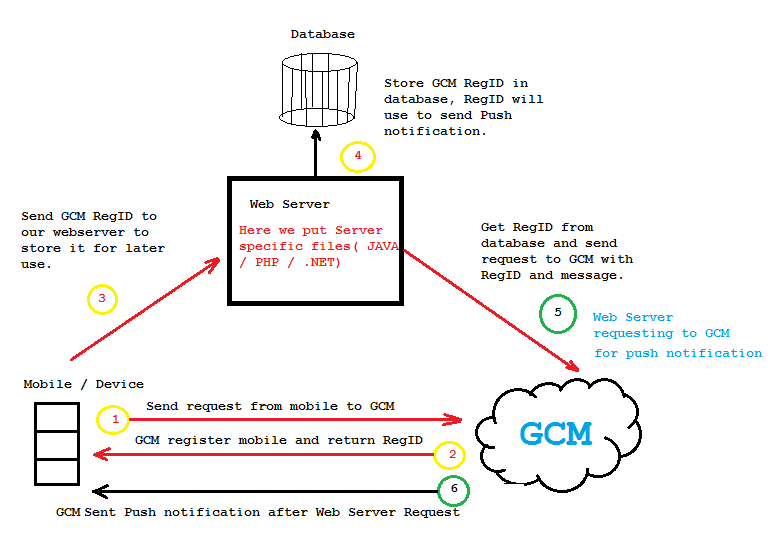
\includegraphics[scale=0.25]{image/gcm.png}
\caption{GCM Working}
\end{figure}

\end{frame}

\begin{frame}
\frametitle{Notification Generated On Android Devices}
\begin{figure}
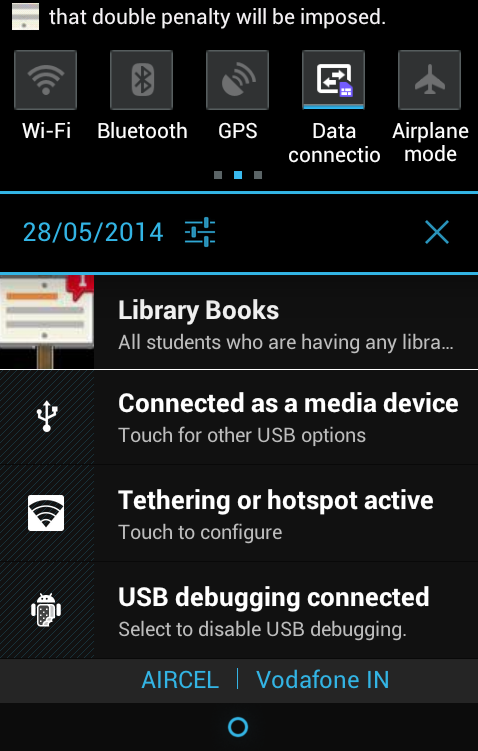
\includegraphics[scale=0.2]{image/notify.png}
\caption{Notification Generated}
\end{figure}
\end{frame}

\section{Technologies Used}
\begin{frame}
\frametitle{Technologies Used}
\begin{itemize}
\item XML\pause
\item Java\pause
\item PHP\pause
\item SQLite \pause
\item MySQL\pause
\end{itemize}
\end{frame}

\subsection{XML}
\begin{frame}
\frametitle{XML}
XML is Extensive Markup Language.Extensible Markup Language (XML) is a markup language that defines a set of rules for encoding documents in a format that is both human-readable and machine-readable.The design goals of XML emphasize simplicity, generality, and usability over the Internet.[6] It is a textual data format with strong support via Unicode for the languages of the world.\\
It is used for designing the layouts of each activity of the application.

\end{frame}

\subsection{Java}
\begin{frame}
\frametitle{Java}
Java is an Object Oriented Programming language used for making Desktop applications, Web Application and Mobile Applications.
Android relies heavily on the JAVA fundamentals. The Android SDK includes many standard Java libraries as well as special Android Libraries that will help you develop awesome Android applications.

\end{frame}

\subsection{PHP}
\begin{frame}
\frametitle{PHP}
PHP (Hypertext Preprocessor) is a widely-used open source general-purpose scripting language that is especially suited for web development and can be embedded into HTML.\\
PHP is used at backend in order to send the requests and receive the responses from the Web Server.


\end{frame}

\subsection{SQLite}
\begin{frame}
\frametitle{SQLite}
SQLite is a relational database management system contained in a C programming library. In contrast to other database management systems, SQLite is not a separate process that is accessed from the client application, but an integral part of it. SQLite is a popular choice as embedded database for local/client storage in application software such as web browsers.\\
SQLite is used in application as locall database of each Android device.

\end{frame}

\subsection{MySQL}
\begin{frame}
\frametitle{MySQL}
MySQL is a relational database for use in web applications, and is a central component of the widely used LAMP open source web application software stack.\\
MySQL is used as Web Server database for storing all the incoming notices.

\end{frame}

\section{System Requirements}
\subsection{Software Requirements}
\begin{frame}
\frametitle{Software Requirements}
\begin{enumerate}
\item \textbf{Java Compiler:}\\
Java compiler is required in order to compile all the Java files of the project.

\item \textbf{ADT Bundle}\\
ADT Bundle stands for Android Development ToolKit. This is an android development environment required to make an 
Android Application.
\end{enumerate}
\end{frame}
\subsection{Hardware Requirements}
\begin{frame}
\frametitle{Hardware Requirements}
\begin{enumerate}
\item \textbf{CPU:} Min. 1.2 GHz
\item \textbf{HDD:} Min. 500MB of free space
\item \textbf{Operating System:} Ubuntu 12.04 or higher.
\item \textbf{Internet Connectivity:} For making connections to Web Server.
\end{enumerate}
\end{frame}


\section{Features of Project}
\begin{frame}
\frametitle{Features of Project}
\begin{itemize}
\item \textbf{Battery Saving Application:} The service implemented in application is not running all the time. Whenever GCM ping the mobile, only then it makes a broadcast to phone that initiates the service. In this way, its saving your device's battery alot.\pause

\item \textbf{Automatically Updated DashBoard:} The dashboard of notice is automatically updated when a new message arrives. the user can himself refresh the dashboard to see any new notice.\pause

\item \textbf{Free Service:} It gives free service to notify all the students. There will be no cost of sending notification to all.
Just have the good system implemented in college and that too free of cost. \pause
\end{itemize}
\end{frame}

\begin{frame}
\frametitle{Features of Project}
\begin{itemize}
\item \textbf{Anytime Anywhere Service:} With this application, notices will be delivered anytime and at any place. There is no restriction of time to send a notice. \pause

\item \textbf{Keeping Notices at one place:} This application allows you to have notices in one place only. If there is an attachment with that, all will be placed in a separate dedicated folder to that application.
\end{itemize}
\end{frame}

\section{Future Scope Of Project}
\begin{frame}
\frametitle{Future Scope Of Project}
\begin{itemize}
\item \textbf{Categorization of Notice:} Notices can be categorized in different categories, so that its possible for user to easily manage the notices.

\item \textbf{Documents and PDF Files:} The attachments can be further improved to include PDF files or Word files.

\item \textbf{Feedback:} Feedback on the notices can also be taken. it can increase communication among the connected members and any issue can be easily sorted out on the spot.
\end{itemize}
\end{frame}

\section{Conclusion}
\begin{frame}
\frametitle{Conclusion}
e-Notice App is going to help a lot in getting updates from college. Every student or staff will be aware of all on going events and activities inside the college. This will lead to make every person well informed about the college.
\end{frame}

\begin{frame}
\begin{center}
\textbf{Thank You}
\end{center}
\end{frame}
\end{document}
